
\section{System Overview}

This demonstration describes a question answering systems that leverages a probabilistic knowledge base.
To introduce this section, we first give a walkthrough of how a question is evaluated.
We then give a detailed description of each component involved in question answering computation.



%We begin with the interface, we describe each of the different methods
%the users has to interact with with the backend knoweldge base.
%We then describe the Logic layer that does translation and of user actions
%to the back end actions. It also allows the user to see the current current
%status of the system.
%We also describe the probabilistic knowledge base driving the system.
%We describe its schema and the integrated functions.

A user user first enters a question \(q\). 
We then leverage the SEMPRE system to translate the question into SPARQL, the de facto language for querying RDF data stores.
The  SQL-like formalism of SPARQL queries produces a set of subgraph expressions as triples.
We can then use the SPARQL query $s(q)$ and extract the supporting triples \(t_{s(q)}\) that underly the subgraph.
These triples are in the form \(\langle s, p, o \rangle\) and correspond to the facts that support the answer to the question.
To obtain the \(t_{s(q)}\), we can evaluate the SPARQL query and materialize each the intermediate triple.
We can use \(t_{s(q)}\) to search our probabilistic knowledge base of facts to obtain the closest matching facts.
Each fact \(f \in \mathcal{F}\) is of the form \(R(A,B)\) and a triple \(t_{s(q)}\) is equivalent to a fact \(f\) when 
\( (s,p,o) = (A,R,B) \).
Given the equivalent facts, we use our k-hop algorithm to determine the joint probability that each fact is correct.
This probability is a truthfulness score that can be paired with each answer to the question.

In the next few sub-sections we describe each part of the process. We start
with the interface where the user can enter natural language questions and a
description of how SEMPRE processes the question (Section~\ref{sec:probqa-interface}).
Next, we describe how we perform lookups for candidate facts (Section~\ref{sec:probqa-search}).
We then define our method to derive the joint probability distribution (Section~\ref{sec:probqa-inference}).


%Our goal is to extract the facts that support the answer to a user's question.
%SPARQL queries describe a sub graph to be matched in the knowedge base.
%We extract the triples sub graps from the SPARQL queries and treat these triples as the facts underlying the answer to the question.
%The algorithm for this is below...


\begin{figure}
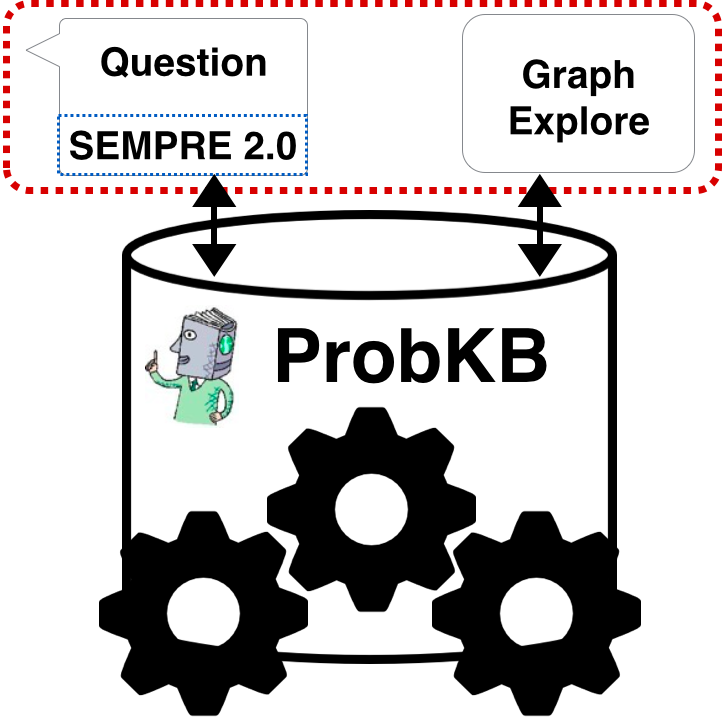
\includegraphics[width=\columnwidth,clip=true,trim=0cm 4cm 0cm 10cm]{images/qaarchitecture.png}
\caption{Question answering system architecture.}
\label{fig:qaarchitecture}
\end{figure}


\subsection{Interface}
\label{sec:probqa-interface}

%The framework is developed using AngularJS\@ to completely compatible with desktop and mobile devices.
The interface allows users to make queries using three different modalities.
Users will be able to enter natural language questions, search through the set of existing facts, and use a graph to explore connections between graphs.
New probabilistic facts and rules can also be added to the system through the interface.
Users can also remove or alter the existing facts and rerun queries.
The status of queries and the underlying processes are displayed on the main interface.

When a user enters a natural language utterance \(q\), we use the SEMPRE 2.0 system to transform the utterance to a logical form~\cite{berant2013freebase,berant2013semantic}.
We then translate the logical form to SPARQL for execution over a knowledge base \(\mathcal{D}\);
let \(s(q,\mathcal{D})\), or equivalently, \(s(q)\) be a function that transforms a natural language utterance to the SPARQL query.
We then parse the SPARQL query and extract the intermediate triples \( t_{s(q)} = \{\langle s,p,o\rangle_1, \ldots \}\). 
Like the SPARQL query, these triples only specify a template of the facts that are required to evaluate the utterance.
We evaluate the SPARQL query over \(\mathcal{D}\) to obtain an answer \( \alpha \), we map the query template to define the candidate set of triples \( t^\alpha_{s(q)} \).

For each triples in \( t^\alpha_{s(q)} \) we perform a look up in \(\mathcal{D'}\) which may or may not be equivalent to the knowledge base \(\mathcal{D'}\).
If there is a exact match, the triple is mapped to a score of 1.
If there is no exact match in \(\mathcal{D}\), we estimate the probability of the triple appearing using a straight-forward application of the chain rule.
The intuition behind this weighting is that if a fact does not exist we would like to compute the probability that the facts could exist.
An equation representing this value is as follows,

\begin{equation}
  \label{eq:probqa-weight}
  \omega(s,p,o) = \begin{cases}
    1 & \mbox{if } exists(\langle s,p,o \rangle) \\ 
    \max( \omega(o,p,s), P(s,p,o)) & \mbox{otherwise,}
  \end{cases}
\end{equation}

where \( P(s,p,o) = P(s|p,o)  P(p|o)  P(o) \).

We then use the K-hop algorithm to estimate the joint probability of a fact existing given the rules.


\begin{lstlisting}[language=Python,basicstyle=\small,showstringspaces=false,mathescape=true,frame=single,numbers=left,label=probqa-algo,caption={Algorithm for obtaining the information}]
def answer (q):
  t ={`q': q,
      `s': SEMPRE.toLogicalForm (q) }
  t[`a'] = SEMPRE.toSPARQL (t[`s'])
  execute ($\mathcal{D}$, t) # Evaluate query
  # Do fact search
  t['$\alpha$'] = findMatches ($\mathcal{D}$, t) 
  t['$\omega$'] = evaluateTriples ($\mathcal{D}$, t) # Equation~\ref{eq:probqa-weight}
  t['khop'] = kHop ($\mathcal{D}$, t['$\alpha$'])

  # TODO Perform a weighted combination of kHop and $\omega$

  return t

\end{lstlisting}


%\begin{algorithm}[ht]
%  \caption{Sequential Gibbs Sampling}
%  \label{alg:gibbs}
%  \begin{algorithmic}[1]
%    \WHILE {done = false}
%    ¦ ¦ ¦ ¦\FOR{i $\leftarrow$ 0 $\KwTo$ numChains}
%    ¦ ¦ ¦ ¦ ¦ \STATE performGibbsStep(i)
%    ¦ ¦ ¦ ¦\ENDFOR
%    ¦ ¦ ¦ ¦ ¦ ¦\IF{burnIn}
%%    ¦ ¦ ¦ ¦ ¦ ¦ ¦ \STATE burnConvergeTest-$>$appendValues(truthValues)
%    ¦ ¦ ¦ ¦ ¦ ¦ ¦ \STATE burnIn $\leftarrow$ checkConvergeAll(burnConvergeTests)
%    ¦ ¦ ¦ ¦ ¦ ¦\ELSE \STATE convergeTest-$>$appendValues(truthValues)
%    ¦ ¦ ¦ ¦ ¦ ¦ ¦ ¦ ¦\STATE done $\leftarrow$ checkConvergeAtLeast(convergeTests)
%    ¦ ¦ ¦ ¦ ¦ ¦\ENDIF
%    \ENDWHILE
%  \end{algorithmic}
%\end{algorithm}




\subsection{Fact Search}
\label{sec:probqa-search}

%Describe how facts are searched using the database.
Given a candidate fact \(f\) of the form \(\langle s, p, o \rangle\), we use the
database to search for the top triples that are similar to \(f\).
Some sets of facts contain blank nodes or expect lists or sets of information.
For example, the utterance ``\texttt{Who are Justin beiber's siblings?}'' produces 
a SPARQL query that contains the following subtriples: (1)  
%Describe how results are ranked.
%Describe how new results are discovered.
%Give algorithm, describe how blank nodes are compressed and other fact cleaning tasks.

%\subsubsection{Graph Exploring}
Describe D3 visualization of graph and rule display
Describe user interaction with graph
Describe user selecting facts
Describe users removing facts


\subsection{Probabilistic Inference}
\label{sec:probqa-inference}
Given that we have a set of matching/partially matching facts, give an explanation of how values from the khop algorithm are evaluated.

We compare the fact probabilities to the sempre results.

\subsubsection{Knowledge Base}

Describe the PostgreSQL database and the other services running on servers.
Describe the tables 
Describe the functions that are called
Describe the parallelism

The system is loaded with docker, a system container, so any modifications by demo can be quickly rolled back to the initial state.





% See other examples: http://www.vldb.org/2014/program/papers/demo/

